\documentclass[11pt]{article}

\usepackage[english]{babel}                 %% hyphenation rules, spell-checker
\usepackage{amsmath,amssymb}                        %% macros like align* and pmatrix
\usepackage{graphicx,epstopdf}              %% for .eps graphs
\usepackage[official]{eurosym}              %% 1 \euro
\usepackage[a4paper,margin=2cm]{geometry}   %% margins
\usepackage{nameref}
\usepackage{hyperref}                       %% hyperlinks to urls
\usepackage{float}                    

\frenchspacing                              %% no extra space after period
\addtolength{\parskip}{0.5\baselineskip}    %% some white space between paragraphs
\setlength{\parindent}{0pt}                 %% but no indentation
\renewcommand{\baselinestretch}{1.1}        %% line spacing of TeX is small
\DeclareMathOperator{\E}{\mathbb{E}}
\DeclareMathOperator{\Var}{\text{Var}}
\DeclareMathOperator{\Cov}{\text{Cov}}


\title{Non-life --- Assignment NL5}  %% don't forget to change!

\author{
  Niels Keizer\footnote{Student number: 10910492}
  \quad and \quad
  Robert Jan Sopers\footnote{Student number: 0629049}
}

\date{\today}

\begin{document}

\maketitle


\section{The Bornhuetter-Ferguson method}

\subsection*{Q18}

We repeat the code from the assignment, then we extract the \verb|alpha| and \verb|beta| values. Then we check if the sum over the past values obtained from \verb|alpha| and \verb|beta| equals the sum over the fitted values. Finally, we calculate the sum over the future estimated values.

\begin{verbatim}
> Xij <- scan(n=36)
1: 156 37  6  5 3 2 1 0
9: 154 42  8  5 6 3 0
16: 178 63 14  5 3 1
22: 198 56 13 11 2
27: 206 49  9  5
31: 250 85 28
34: 252 44
36: 221
Read 36 items
> TT <- 8; i <- rep(1:TT, TT:1); j <- sequence(TT:1); k <- i+j-1
> fi <- as.factor(i); fj <- as.factor(j); fk <- as.factor(k)
> ee <- c(28950,29754,31141,32443,34700,36268,37032,36637)
> Expo <- rep(ee, TT:1)
> CL <- glm(Xij~fi+fj, quasipoisson)
> EE <- glm(Xij~offset(log(Expo))+fj, quasipoisson)
> 
> cc <- exp(coef(CL))
> alpha <- cc[1] * c(1,cc[2:8]); names(alpha)[1] <- "fi1"
> beta <- c(1,cc[9:15]); names(beta)[1] <- "fj1"
> alpha <- alpha * sum(beta); beta <- beta / sum(beta)
> 
> i_tot <- rep(1:8, each=8)
> j_tot <- rep(1:8,8)
> k_tot <- i_tot+j_tot-1
> future <- k_tot>8
> 
> sum(CL$fitted.values)
[1] 2121
> sum(alpha[i_tot]*beta[j_tot]*!future)
[1] 2121
> sum(alpha[i_tot]*beta[j_tot]*future)
[1] 152.0312
\end{verbatim}

We see that the \verb|alpha| and \verb|beta| give the same past value as the model itself. We also see that we get the results that the assignment says we should get.

The total of the fitted values for past observations equals \verb|sum(Xij)| because of the marginal totals property.

\subsection*{Q19}

We run the code from the assignment and get the following result in \verb|R|.

\begin{verbatim}
> round(tapply(fitted.values(EE)-Xij,j,sum),6)
1 2 3 4 5 6 7 8 
0 0 0 0 0 0 0 0 
\end{verbatim}

The statement in \verb|R| is a sum over the difference between the observed and the fitted values for equal \verb|j|. These are the column sums. Because the \verb|EE| method uses dummy variables for the columns, the marginal totals property holds for the column sums.

\subsection*{Q20}

We execute the following code in \verb|R|, where we replace the dots by \verb|sum(fits) - sum(Xij)|.

\begin{verbatim}
> reserves <- numeric(); lasts <- c(171,181,191,201,211,271,261,251,241,231,221)
> for (last in lasts){
+   Xij[36] <- last
+   cc <- exp(coef(glm(Xij~fi+fj,quasipoisson)))
+   alpha <- c(1,cc[2:TT])*cc[1]; beta <- c(1,cc[(TT+1):(2*TT-1)])
+   fits <- (alpha %o% beta)
+   reserve <- sum(fits) - sum(Xij) ## the sum of the 'future' fitted values
+   reserves <- c(reserves, reserve) 
+ }
> rbind(lasts, reserves=round(reserves))
         [,1] [,2] [,3] [,4] [,5] [,6] [,7] [,8] [,9] [,10] [,11]
lasts     171  181  191  201  211  271  261  251  241   231   221
reserves  132  136  140  144  148  172  168  164  160   156   152
> plot(lasts, reserves); lines(range(lasts),range(reserves))
\end{verbatim}

This results in the following plot:

\begin{figure}[H]\label{fig:q20}
	\centering
	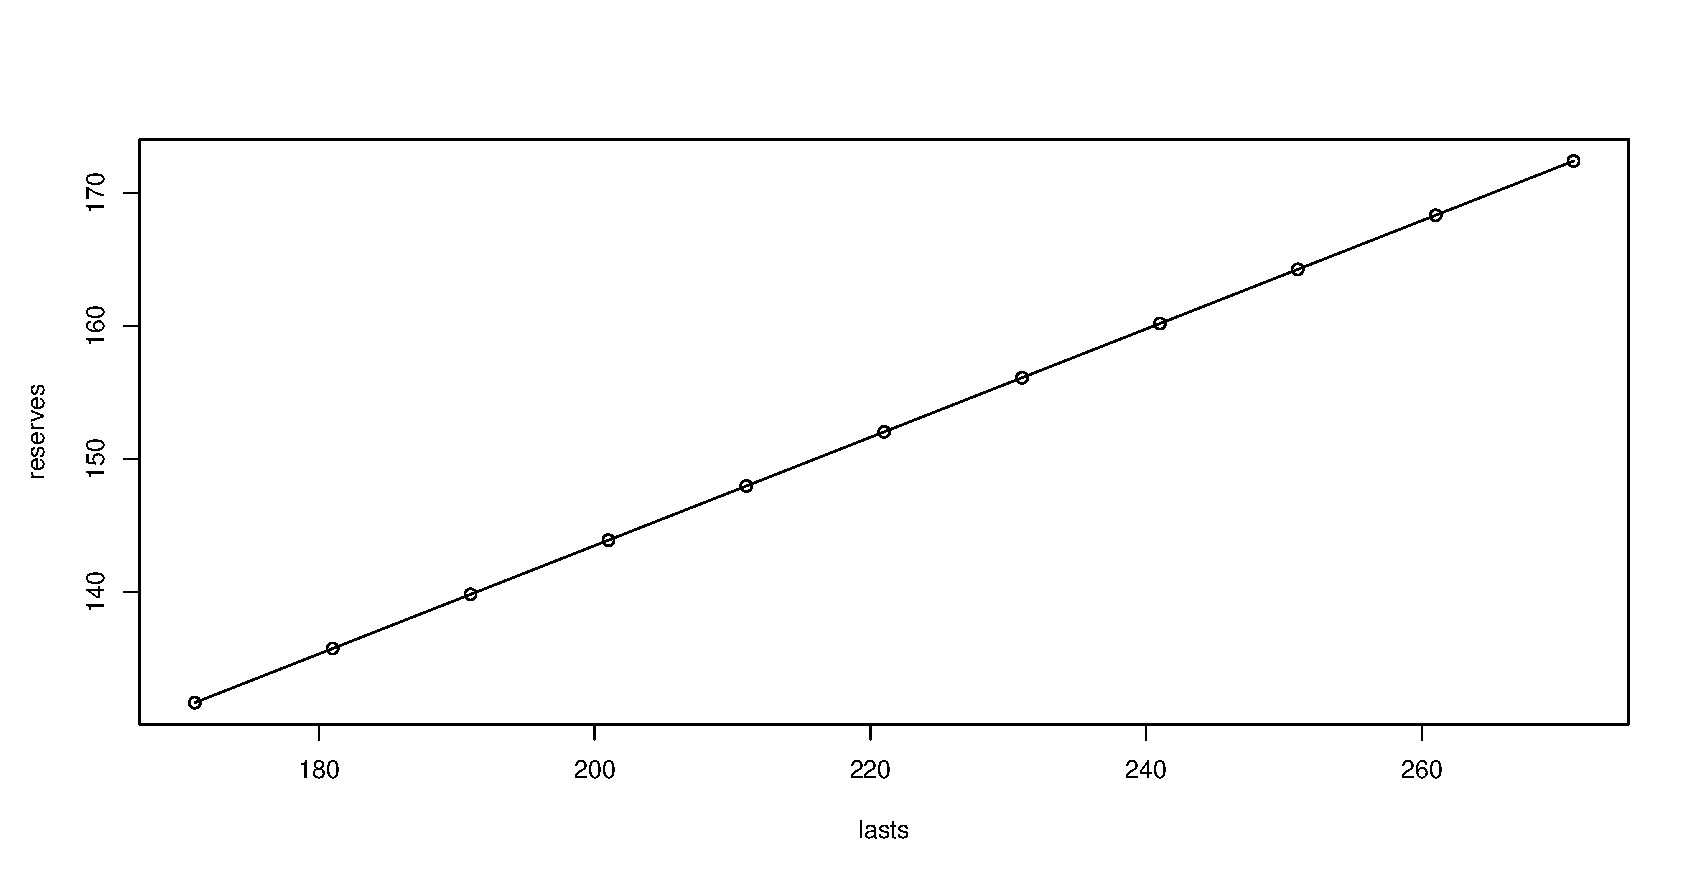
\includegraphics[width=0.8\textwidth]{fig_q20.eps}
	\caption{A plot of the chain ladder reserves against the last claim total.}
\end{figure}

\subsection*{Q21}

First we check the quality of a linear fit in \verb|R|.

\begin{verbatim}
> lin_fit <- lm(reserves~lasts)
> summary(lin_fit)

Call:
lm(formula = reserves ~ lasts)

Residuals:
Min         1Q     Median         3Q        Max 
-5.293e-12 -2.053e-12  7.766e-13  1.608e-12  5.461e-12 

Coefficients:
             Estimate Std. Error   t value Pr(>|t|)    
(Intercept) 6.198e+01  7.372e-12 8.409e+12   <2e-16 ***
lasts       4.074e-01  3.302e-14 1.234e+13   <2e-16 ***
---
Signif. codes:  0 ‘***’ 0.001 ‘**’ 0.01 ‘*’ 0.05 ‘.’ 0.1 ‘ ’ 1

Residual standard error: 3.463e-12 on 9 degrees of freedom
Multiple R-squared:      1,	Adjusted R-squared:      1 
F-statistic: 1.523e+26 on 1 and 9 DF,  p-value: < 2.2e-16
\end{verbatim}

From these results, we conclude that a linear fit is just about perfect.

We consider the final steps from Verbeek's algorithm for computing the CL coefficients. From the row sums, we see that $\alpha_{8}\beta_{1} = X_{8,1}$ ($X_{8,1} = R_{8}$). Because $\sum_{j} \beta_{j} = 1$ and the $\beta_{j}$ values have already been determined for $j \in (2, \ldots, 8)$, $\beta_{1}$ is independent from $X_{8,1}$. This implies $\alpha_{8} = X_{8,1}/\beta_{8}$, thus $\alpha_{8}$ is linearly dependent on $X_{8,1}$. By construction, all predicted values on row 8 are now also linearly dependent on $X_{8,1}$ and so is their sum. The total reserve is the sum of all predicted values, from which then follows that there is a linear relation between $X_{8,1}$ and the reserve.

We know that the sum over the predicted values of rows 1 to 7 are independent from $X_{8,1}$ and should therefore equal the intercept. We check this in \verb|R|.

\begin{verbatim}
> lin_fit$coefficients[1]
(Intercept) 
   61.98482 
> sum(alpha[1:7] %o% beta)-sum(Xij[i<=7])
[1] 61.98482
\end{verbatim}


\subsection*{Q22}

We construct the vector $\hat{M}$ with the following code:

\begin{verbatim}
M <- ee / ee[1] * alpha[1]
\end{verbatim}

\subsection*{Q23}

We copy the code from the assignment and fill the dots to obtain the following in \verb|R|.

\begin{verbatim}
> i_tot <- rep(1:8, each=8);j_tot <- rep(1:8,8)
> pred.CL <- alpha %*% t(beta); round(pred.CL, 4)
          fj1     fj2     fj3    fj4    fj5    fj6    fj7 fj8
[1,] 149.2060 40.2450 10.0252 5.2008 3.0131 1.8192 0.4907   0
[2,] 154.8901 41.7781 10.4071 5.3989 3.1279 1.8885 0.5093   0
[3,] 188.0126 50.7122 12.6327 6.5535 3.7968 2.2923 0.6183   0
[4,] 201.1539 54.2567 13.5156 7.0115 4.0622 2.4526 0.6615   0
[5,] 196.0964 52.8926 13.1758 6.8352 3.9600 2.3909 0.6448   0
[6,] 271.5200 73.2364 18.2436 9.4643 5.4832 3.3105 0.8929   0
[7,] 233.1209 62.8791 15.6635 8.1258 4.7077 2.8423 0.7666   0
[8,] 221.0000 59.6098 14.8491 7.7033 4.4630 2.6945 0.7267   0
> pred.BF <- M %*% t(beta); round(pred.BF, 4)
          fj1     fj2     fj3    fj4    fj5    fj6    fj7 fj8
[1,] 149.2060 40.2450 10.0252 5.2008 3.0131 1.8192 0.4907   0
[2,] 153.3498 41.3626 10.3036 5.3452 3.0968 1.8697 0.5043   0
[3,] 160.4983 43.2908 10.7840 5.5944 3.2412 1.9569 0.5278   0
[4,] 167.2087 45.1008 11.2348 5.8283 3.3767 2.0387 0.5499   0
[5,] 178.8411 48.2383 12.0164 6.2338 3.6116 2.1805 0.5881   0
[6,] 186.9225 50.4181 12.5594 6.5155 3.7748 2.2790 0.6147   0
[7,] 190.8600 51.4802 12.8240 6.6527 3.8543 2.3270 0.6276   0
[8,] 188.8242 50.9311 12.6872 6.5818 3.8132 2.3022 0.6209   0
> future <- xtabs(i_tot+j_tot-1>8~i_tot+j_tot)
> reserve.CL <- sum(pred.CL*future)
> reserve.BF <- sum(pred.BF*future)
> reserve.CL;reserve.BF
[1] 152.0312
[1] 125.9025
\end{verbatim}

We see that the reserve from the CL method is higher than the reserve from the BF method.

\end{document}
